% Copyright 2015 by Fabien Lahoudere <fabienlahoudere.pro@gmail.com>.
% !TEX TS-program = pdflatex
% !TEX encoding = UTF-8 Unicode

\documentclass{beamer}

\mode<presentation>
{
  \usetheme{Warsaw}
  \setbeamercovered{transparent}
}

\usepackage[english]{babel}
\usepackage[utf8]{inputenc}
\usepackage{times}
\usepackage[T1]{fontenc}
\usepackage{listingsutf8}
\usepackage{marvosym} % \MVRIGHTarrow

\definecolor{light-gray}{gray}{0.95}
\definecolor{light-blue}{RGB}{20,20,80}
\lstdefinestyle{customc}{language=C,
	breaklines=true,
	frame=L,
	xleftmargin=\parindent,
	showstringspaces=false,
	numbersep=5pt,
	tabsize=8,
	backgroundcolor=\color{light-gray},
	frame=shadowbox,
	rulesepcolor=\color{blue!40!white},
	basicstyle=\ttfamily\tiny,
	numberstyle=\tiny,
    keywordstyle=\bfseries\color{green!40!black},
    commentstyle=\itshape\color{purple!40!black},
    identifierstyle=\color{blue},
    stringstyle=\selectfont\color{orange}}

\lstdefinestyle{customshell}{language=bash,
	belowcaptionskip=1\baselineskip,
	basicstyle=\ttfamily\tiny}


\title[Linux (Généralités)]
{Généralités sur Linux}

\author[Fabien Lahoudère]
{Fabien Lahoudère}

\institute[Open Wide]
{
  Consultant Linux embarqué chez Open Wide\\
  fabienlahoudere.pro@gmail.com\\
  aragua sur github et IRC
}

\date[Mai 2015]
{INSA Linux embarqué, Novembre 2015}

\subject{Debug Linux embarqué}

\AtBeginSubsection[]
{
  \begin{frame}<beamer>{}
    \tableofcontents[currentsection,currentsubsection]
  \end{frame}
}


%%%%%%%%%%%%%%%%%%%%%%%    DOCUMENT    %%%%%%%%%%%%%%%%%%%%%%%
\begin{document}

\begin{frame}
  \titlepage
\end{frame}

\begin{frame}{Sommaire}
  \tableofcontents
\end{frame}

%%%%%%%%%%%%%%%%%%%%%%%    Intro    %%%%%%%%%%%%%%%%%%%%%%%
\section{Introduction}

\subsection{OE}
\begin{frame}{Linux}{OE}
	OE est un « framework de compilation croisée » démarré par Chris Larson en 2003 pour OpenZaurus (Zaurus = le « premier » PDA sous Linux)\\
	
\end{frame}

\subsection{Linux dans l'industrie}
\begin{frame}{Linux}{Linux dans l'industrie}
	Linux s'est en premier imposé dans le monde de l'entreprise sous forme de systèmes d'exploitations sur serveur.\\
	Peu de temps après Linux fut adapté aux mondes des systèmes embarqués.\\
	L'intérét pour les entreprise est:
	\begin{itemize}
		\item
			de maitriser les sources de leur OS.\\
		\item
			d'économiser le prix des licences.\\
		\item
			de bénéficier du support d'une communauté importante de développeur.\\
	\end{itemize}
	Seule la partie Desktop a du mal à émmergé face à ses concurrents.\\
\end{frame}

%%%%%%%%%%%%%%%%%%%%%%%    Concept    %%%%%%%%%%%%%%%%%%%%%%%
\section{Concepts}

\begin{frame}{Concepts}{Basé sur UNIX}
	Implémentation libre d'UNIX diffusé sous licence GPL\\
	Inspiré des deux versions: AT\&T et BSD\\
	Les principes d'UNIX sont respectés:
	\begin{itemize}
		\item
			Simplicité, modularité, respect des standards, ouverture
		\item
			Deux espaces de mémoire: noyau / utilisateur
		\item
			Le noyau permet d'accéder au matériel (pilotes, appels système)
		\item
			Tout composant est un fichier: répertoire, périphérique, élément de communication, etc. (organisation arborescente)
		\item
			Puissance de la «ligne de commande» (shell et regexpr)			
	\end{itemize}	
\end{frame}

\begin{frame}{Concepts}{Fonctionnalitées}
	\begin{itemize}
		\item
			Noyau monolithique (en un seul fichier) + modules dynamiques
		\item
			Création des processus via fork() et exec()
		\item
			Multi-threading
		\item
			Nombreuses piles réseau (IPv4, IPv6, Ethernet, etc.)
		\item
			Organisation des fichiers arborescente à partir de la racine (/), montage et démontage logique (mount)
		\item
			Notion de super-utilisateur (root), groupes, et utilisateurs
	\end{itemize}
\end{frame}

%%%%%%%%%%%%%%%%%%%%%%%    License    %%%%%%%%%%%%%%%%%%%%%%%
\section{Licence}

\begin{frame}{GPL en bref}{}
	GPL General Public License \\
	On la surnomme également copyleft \\
	La GPL v2 (1991) est la plus répandue (ex: noyau Linux)\\
	La licence s'applique uniquement en cas de redistribution\\
	Un code source utilisant du code GPL est du travail dérivé et doit être publié\\
	Publication: celui qui reçoit la version binaire peut obtenir le code source\\
	Pas de lien (ld) possible entre du code GPL et du code propriétaire
\end{frame}

\begin{frame}{LGPL}{}
	La GPL est complexe à gérer dans l'industrie \MVRightarrow{} création de la LGPL \\
	Le lien avec du code propriétaire est possible avec la LGPL (Lesser/Library GPL) !\\
	En majeure partie, les bibliothèques système sont diffusées sous LGPL (exemple: GNU-libc)\\
	Dans le cas d'une application propriétaire il faut donc vérifier qu'aucune bibliothèque liée n'est GPL\\
	Le lien dynamique n'affranchit pas de la licence sauf dans des cas très particuliers\\
\end{frame}

\begin{frame}{GPL uniquement pour LINUX}{}
	Dans l'espace noyau (pilotes), SEULE la GPL s'applique (en théorie) !\\
	En théorie: On ne peut utiliser les headers du noyau Linux pour créer des binaires noon GPL\\
	Certaines fonctions ne sont pas disponibles si la licence n'est pas GPL\\
	En pratique: tolérance si le pilote n'a pas été créé pour Linux (cas du portage) => nVidia, Broadcom, ...\\
	Cependant les pilotes binaires posent des soucis techniques vu qu'un pilote fonctionne pour la version de noyau utilisée pour la compilation\\
\end{frame}

\begin{frame}{GPL V3}{}
	Nouvelle version sortie en 2007\\
	Oblige à fournir les éléments pour construire un logiciel fonctionnel => réponse à la Tivoisation\\
	La GPL v2 demande uniquement la publication des sources à celui qui a reçu le binaire\\
	La GPL v3 ne sera pas utilisée pour le noyau Linux.\\
	Voir: http://www.gnu.org/licenses/quick-guide-gplv3.fr.html\\
\end{frame}


\section{Architecture GNU/Linux}

\begin{frame}{Architecture}{Système GNU/Linux}
	Linux est un noyau. Seul il ne sert à rien. On parlera donc de système GNU/Linux.
	Il est en général composé de:
	\begin{itemize}
		\item
			Un bootloader (Rare sont les carte capable de booter un noyau Linux)\\
			Il est trop gros et doit etre chargé en RAM (elle doit etre initialisé par un microcode)
		\item
			Le noyau Linux (gérant les ressources de la machine)
		\item
			Un système de fichier contenant à minima un programme de démarrage (rootfs)
	\end{itemize}
\end{frame}

\begin{frame}{Architecture}{Système GNU/Linux}
	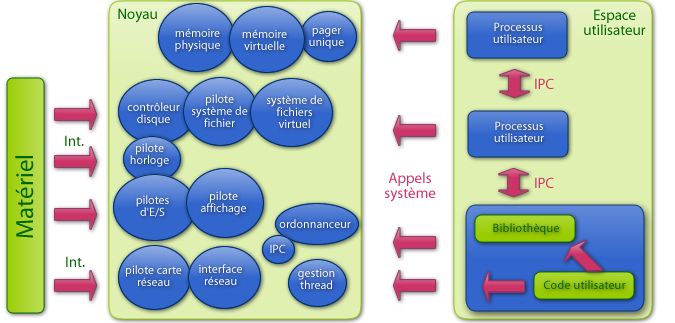
\includegraphics[width=10cm]{system_arch.png}
\end{frame}

\subsection{Noyau}
\begin{frame}{Architecture}{Noyau}
	Le noyau Linux est un binaire de type ELF.\\
	Son image est souvent compréssé pour gagner en taille lors du déploiement et de la copie en RAM\\
	Il contient un auto extracteur qui va le décomprésser\\
	Fournit des services nécéssaires à sa fonction:
	\begin{itemize}
		\item
			ordonanceur
		\item
			gestion mémoire, disque, interface réseaux
		\item
			service abtraits (systeme de fichier, pile réseaux ...)
	\end{itemize}
	Une grande partie du noyau peut etre déporté en module chargé dynamiquement.
\end{frame}

\begin{frame}{Architecture}{Noyau}
	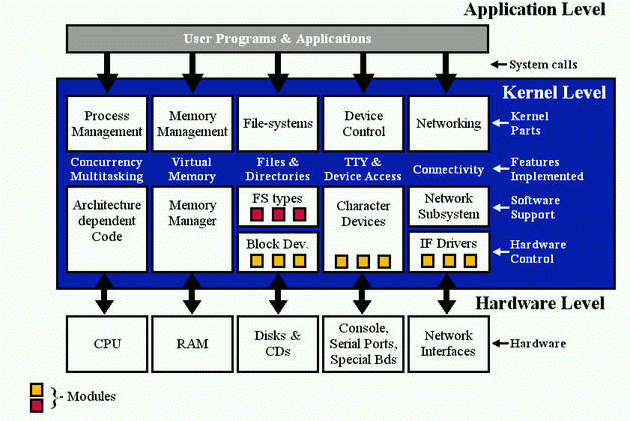
\includegraphics[width=10cm]{kernel_arch.png}
\end{frame}

\begin{frame}{Architecture}{Module noyau}
	Modules noyau: .ko (Kernel Object)\\
	Les modules binaires sont liés à la version du noyau !\\
	Peut se compiler après Nécéssite les entetes du noyau\\
	Mécanisme système pour charger les modules dynamiquement: modprobe, insmod, rmmod
\end{frame}

\subsection{Rootfs}

\begin{frame}{Architecture}{Organisation d'un rootfs}
	Organisation commune à 90\% entre les UNIX
	Quelques spécificités GNU/Linux et distribution
	Les fichiers communs:
	\begin{itemize}
		\item
			/bin,/sbin,/usr/bin,/usr/sbin: binaires communs et systèmes
		\item
			/lib,/usr/lib: bibliothèques et modules noyau
		\item
			/etc: fichiers de configuration
		\item
			/dev: nœuds d'accès aux périphériques (nodes)
		\item
			/var: fichiers variables: log, spool, mail, ...
		\item
			/opt: pour les programmes externes (ex: OpenOffice)
		\item
			/home: accueille les répertoires des utilisateurs
	\end{itemize}
\end{frame}

\begin{frame}{Architecture}{Organisation d'un rootfs}	
	Quelques répertoires spéciaux:
	\begin{itemize}
		\item
			/lib/modules: contient les modules du noyau
		\item
			/root: home-directory de l'utilisateur root (pas dans OE)
		\item
			/media: point de montage des volumes amovibles
		\item
			/proc: système de fichier virtuel (état du système)
		\item
			/sys: idem pour les périphériques connectés (2.6)
		\item
			/boot: noyau statique (vmlinuz, uImage, ...)
	\end{itemize}
\end{frame}

\begin{frame}{Architecture}{/proc}
	Système de fichier virtuel (lecture/écriture) géré par le noyau. (Réponse sur solicitation, pas d'écriture sur un support)\\
	Intérêt: manipuler les variables systèmes comme de fichiers (cat, echo, grep)\\
	Exemples:
	\begin{itemize}
		\item
			/proc/version: version du noyau
		\item
			/proc/cpuinfo: type(s) de processeur(s)
		\item
			/proc/interrupts: interruptions
		\item
			/proc/pid: répertoire décrivant le processus associé au pid
		\item
			/proc/mounts: partitions montées
		\item
			/proc/modules: liste des modules noyau chargés
	\end{itemize}
	Nombreuses commandes systèmes basé sur /proc : lsmod, lspci, top, mount, ...
	Il est aisé de proposer une entrée dans /proc dans un nouveau module grâce à une API
\end{frame}

\begin{frame}{Architecture}{/sys}
	Introduit dans le noyau 2.6 (2003) => sysfs\\
	Vue synthétique des périphériques connectés\\
	\begin{itemize}
		\item
			/sys/class (utilisé par UDEV)
		\item
			/sys/modules
		\item
			/sys/bus
	\end{itemize}		
	But: mieux gérer l'ajout/suppression dynamique des périphériques (hotplug)
	Utilisé par UDEV pour créer dynamiquement les entrées dans /dev 
	Quelques recouvrements avec /proc (bus PCI, USB, ...)
\end{frame}

\end{document}
